% Theorem 10's bipartite graph, for one client j with m=3, k=1 (so m-k=2 rejection slots).
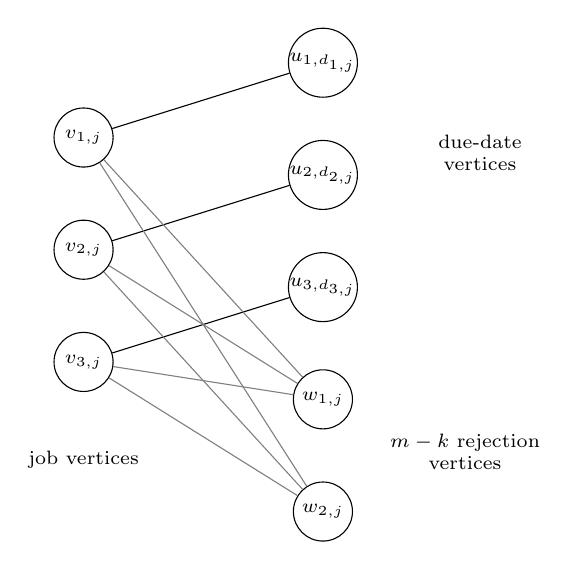
\begin{tikzpicture}[scale=0.95,every node/.style={circle,draw,minimum size=0.75cm,inner sep=0pt,font=\scriptsize}]

\node (v1) at (0,3) {$v_{1,j}$};
\node (v2) at (0,1.5) {$v_{2,j}$};
\node (v3) at (0,0) {$v_{3,j}$};

\node (u1) at (3.2,4) {$u_{1,d_{1,j}}$};
\node (u2) at (3.2,2.5) {$u_{2,d_{2,j}}$};
\node (u3) at (3.2,1) {$u_{3,d_{3,j}}$};
\node (w1) at (3.2,-0.5) {$w_{1,j}$};
\node (w2) at (3.2,-2) {$w_{2,j}$};

\draw (v1) -- (u1);
\draw (v2) -- (u2);
\draw (v3) -- (u3);
\foreach \v in {v1,v2,v3}
  \foreach \w in {w1,w2}
    \draw[gray] (\v) -- (\w);

\node[draw=none,font=\scriptsize] at (0,-1.3) {job vertices};
\node[draw=none,font=\scriptsize] at (3.2,2.9) [anchor=west] {};
\node[draw=none,font=\scriptsize,align=center] at (5.3,2.8) {due-date\\vertices};
\node[draw=none,font=\scriptsize,align=center] at (5.1,-1.2) {$m-k$ rejection\\vertices};

\end{tikzpicture}
